\documentclass[slidestop,compress, 10pt]{beamer}

%\usepackage{beamerthemesplit}
\graphicspath{{Figures/}}
%\usetheme[height=1cm]{Rochester}
%\usetheme[height=1cm]{Singapore}
%\usetheme{Boadilla}
%\usetheme{boxes}
\usetheme[]{Boadilla} %secheader
%\useoutertheme[footline=authortitle,subsection=false,height=1cm]{miniframes}
%\useoutertheme[subsection=false,height=1cm]{smoothbars}
\usepackage{epic}
%\usepackage{natbib}
%\usepackage[notocbib]{apalike}
\usepackage{color}
\beamertemplatenavigationsymbolsempty
\usepackage{graphicx}
\usepackage{color}
\usepackage[mathscr]{eucal}
\usepackage{epsfig}
\usepackage[all]{xy}
\usepackage{url}
\usepackage{setspace}
%\usepackage{xmpmulti}
\DeclareMathOperator{\E}{E}
\DeclareMathOperator{\I}{I}
\DeclareMathOperator{\Var}{Var}
\DeclareMathOperator{\Cov}{Cov}
\DeclareMathOperator{\logit}{logit}
\DeclareMathOperator{\dom}{dom}
\DeclareMathOperator{\cl}{cl}
\DeclareMathOperator{\bd}{bd}
\DeclareMathOperator{\rbd}{rbd}
\DeclareMathOperator{\intr}{int}
\DeclareMathOperator{\rint}{rint}
\DeclareMathOperator{\con}{con}
\DeclareMathOperator{\pos}{pos}
\DeclareMathOperator{\aff}{aff}
\DeclareMathOperator{\epi}{epi}
\DeclareMathOperator{\lev}{lev}
\DeclareMathOperator{\spanl}{span}

\def\RR{{\mathbb R}}
\def\ZZ{{\mathbb Z}}
\def\DD{{\mathcal D}}
\def\XX{{\mathcal X}}
\def\YY{{\mathcal Y}}
\def\TT{{\mathcal T}}
\def\NN{{\mathcal N}}
\newcommand{\deriv}[2]{\frac{d #1}{d #2}}
\newcommand{\dderiv}[2]{\frac{d^2 #1}{d #2^2}}
\newcommand{\pderiv}[2]{\frac{\partial #1}{\partial #2}}
\newcommand{\ppderiv}[2]{\frac{\partial^2 #1}{\partial #2^2}}
\newcommand{\ppmderiv}[3]{\frac{\partial^2 #1}{\partial #2 \partial #3}}
\newcommand{\fatdot}{\,\cdot\,}
\newcommand{\inner}[1]{\langle #1 \rangle}
\newcommand{\set}[1]{\{\, #1 \,\}}
\newcommand{\abs}[1]{\lvert #1 \rvert}
\newcommand{\norm}[1]{\lVert #1 \rVert}
\newcommand{\etaMLE}{\hat{\eta}_{\textrm{MLE}}}
\newcommand{\betaMLE}{\hat{\beta}_{\textrm{MLE}}}
\newcommand{\thetaLCM}{\hat{\theta}_{\textrm{LCM}}}
\newcommand{\etaLCM}{\hat{\eta}_{\textrm{LCM}}}
\newcommand{\yobs}{y_{\text{obs}}}
\newcommand{\Gammalim}{\Gamma_{\textrm{lim}}}
\newcommand{\CLCM}{C_{\textrm{LCM}}}

%\setbeamercovered{transparent}

\title{Parameter Estimation in Social Network Models}
\author{
  Saisuke Okabayashi 
%  Charles J. Geyer
}

\institute{Department of Statistics \\ University of Minnesota}

\date{April 5, 2011}


\begin{document}
%\usefoottemplate{\vbox{\tinycolouredline{structure!75}{\color{white}\textbf{\insertauthor\hfill}}\tinycolouredline{structure}{\color{white}\textbf{\inserttitle}\hfill}}}

\frame{\titlepage}
\section{Background}
\frame{
	\frametitle{My research is about}
\begin{itemize}
\item optimization
\item curvature condition
\item linear programming
\item relative boundaries of convex hulls
\item directions of recession
\end{itemize}
\vspace{1in}
\pause
{\textbf{But that's not how it began!} }
}


\frame
{
  \frametitle{It began with some monks ...}
\begin{figure}
\begin{center} 
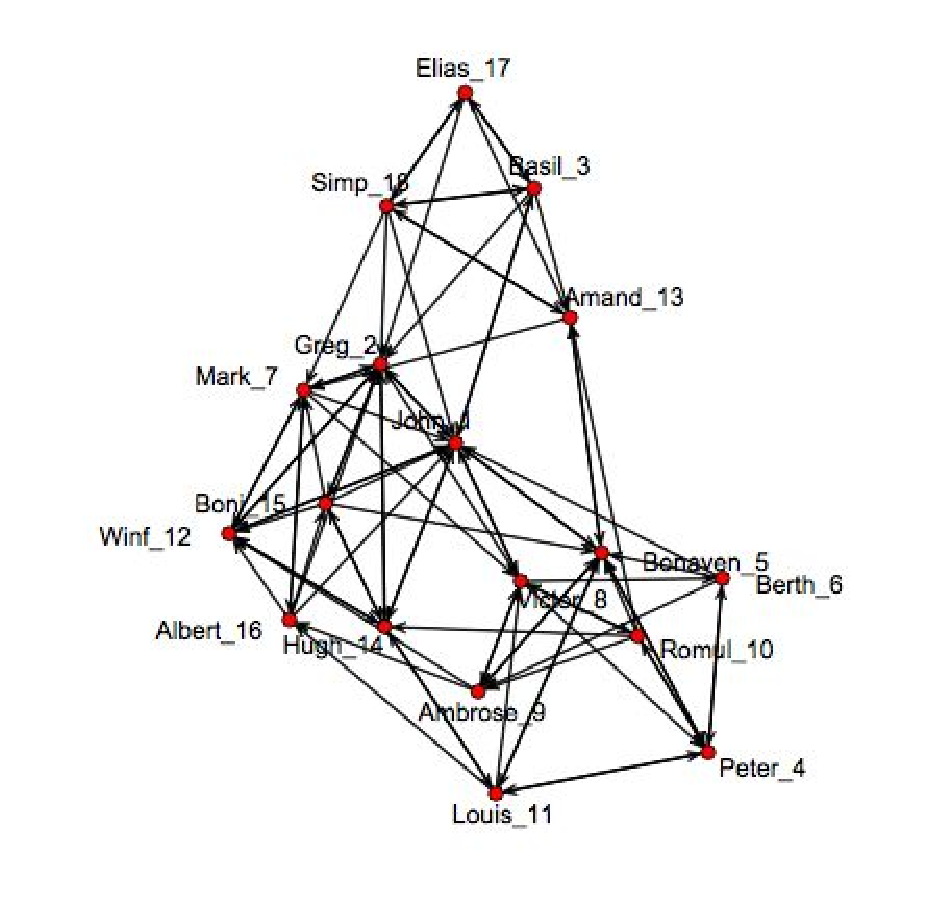
\includegraphics[height=2.8in]{samplike}
\caption{Sampson's (1969) monastery affinity network among 18 monks.} 
\end{center} 
\end{figure}
}
%\frame
%{
%  \frametitle{and... }
%
%\begin{figure}
%\begin{center} 
%\includegraphics[height=2.7in]{florentine}
%\caption{Padgett's (1994) Florentine marriage network among 16 Florentine families around 1430.} 
%\end{center} 
%\end{figure}
%}
\frame
{
  \frametitle{and... }
\begin{figure}
\begin{center} 
\includegraphics[height=2.7in]{fmh-gradesex2}
\caption{National Longitudinal Study of Adolescent Health friendship network of 1,461 students in grades 7 -- 12 without isolates.  Squares=Boys, Circles=Girls.} 
\end{center} 
\label{fmh} 
\end{figure}
}
\frame
{
  \frametitle{and...}

\begin{figure}
\begin{center} 
\includegraphics[height=2.6in]{ecoli}
\caption{\textit{E. Coli} transcriptional regulation network of Shen-Orr et al. (2002).  
Nodes are operons, $i \to j$ indicates that $i$ encodes transcription factor that regulates $j$.} 
\end{center} 
\end{figure}
}

\frame
{
\frametitle{Why networks?}
Networks are a conduit for \emph{flow}.  
\vspace{2mm}

Flow can be:
\begin{itemize}
\item friendship
\item diseases
\item needle-sharing
\item money
\item data
\item airplanes
\item commodities
\item ideas
\item advice 
\item association (among terrorists)
\item binding (between proteins)
\end{itemize}
\vspace{2mm}

\textbf{Goal of a network model: explain the mechanism of this flow.} 
}

%%%%%%%%%%%%%%%%%%%%%%%%%%%%%%%%%%%%%%%%%%%%%%%%%%%%%%%%%%%%%
\section{Modeling}
\frame
{
\frametitle{A network, mathematically}
%\setbeamercovered{transparent}

A social network is a collection of \emph{actors} and the \emph{relations} between each pair of actors.  

We can represent a network with $n$ actors as an $n \times n$ matrix $Y$, where each entry
\begin{align*}
	Y_{ij} =
	\begin{cases} 	1 \quad \text{if a relation exists from actor $i$ to actor $j$}\\
					0 \quad \text{otherwise}
	\end{cases}
\end{align*}
\pause

The Sampson monastery network (directed), in matrix form:
{\tiny
\begin{table}[ht]
\begin{center}
\begin{tabular}{rrrrrrrrrrrrrrrrrr}
  \hline
0 & 1 & 1 & 0 & 1 & 0 & 1 & 0 & 0 & 0 & 1 & 0 & 0 & 0 & 1 & 0 & 0 & 0 \\ 
0 & 0 & 1 & 0 & 1 & 1 & 0 & 0 & 1 & 0 & 0 & 0 & 0 & 0 & 1 & 0 & 0 & 0 \\ 
0 & 1 & 0 & 0 & 0 & 0 & 1 & 1 & 0 & 0 & 0 & 0 & 0 & 1 & 0 & 0 & 0 & 0 \\ 
0 & 1 & 1 & 0 & 1 & 0 & 0 & 0 & 1 & 0 & 0 & 0 & 0 & 0 & 0 & 0 & 0 & 0 \\ 
1 & 1 & 0 & 1 & 0 & 1 & 0 & 0 & 0 & 0 & 0 & 0 & 0 & 0 & 0 & 0 & 0 & 0 \\ 
0 & 1 & 0 & 0 & 1 & 0 & 1 & 0 & 0 & 0 & 1 & 0 & 0 & 1 & 0 & 0 & 0 & 0 \\ 
1 & 0 & 1 & 1 & 1 & 0 & 0 & 0 & 1 & 1 & 0 & 0 & 0 & 0 & 0 & 0 & 0 & 0 \\ 
0 & 0 & 0 & 0 & 0 & 0 & 0 & 0 & 1 & 1 & 1 & 0 & 1 & 0 & 0 & 0 & 0 & 0 \\ 
0 & 1 & 0 & 0 & 0 & 0 & 1 & 1 & 0 & 1 & 1 & 0 & 0 & 0 & 0 & 1 & 0 & 0 \\ 
0 & 0 & 0 & 0 & 0 & 0 & 0 & 1 & 1 & 0 & 1 & 1 & 1 & 0 & 0 & 0 & 0 & 0 \\ 
0 & 0 & 0 & 0 & 0 & 1 & 0 & 1 & 1 & 1 & 0 & 1 & 0 & 0 & 0 & 0 & 0 & 0 \\ 
0 & 1 & 0 & 0 & 0 & 0 & 0 & 1 & 1 & 1 & 1 & 0 & 1 & 0 & 0 & 0 & 0 & 0 \\ 
0 & 0 & 0 & 0 & 0 & 0 & 1 & 1 & 1 & 1 & 0 & 0 & 0 & 1 & 0 & 0 & 0 & 0 \\ 
0 & 0 & 0 & 0 & 0 & 0 & 0 & 1 & 1 & 1 & 0 & 1 & 1 & 0 & 0 & 0 & 0 & 0 \\ 
0 & 1 & 0 & 0 & 0 & 0 & 0 & 0 & 0 & 0 & 0 & 0 & 1 & 0 & 0 & 0 & 0 & 1 \\ 
0 & 0 & 0 & 0 & 0 & 0 & 0 & 0 & 1 & 1 & 0 & 0 & 0 & 0 & 1 & 0 & 1 & 1 \\ 
0 & 0 & 0 & 0 & 0 & 0 & 0 & 0 & 0 & 1 & 0 & 0 & 0 & 0 & 1 & 1 & 0 & 1 \\ 
0 & 0 & 0 & 0 & 0 & 0 & 0 & 0 & 1 & 1 & 0 & 0 & 1 & 0 & 1 & 1 & 1 & 0 \\ 
   \hline
\end{tabular}
\end{center}
\end{table}}
}
\frame
{
\frametitle{01101010001 ...}
Take this matrix and represent element with 0 as white, 1 as Black.
\pause
\begin{columns}[T]
\begin{column}[T]{0.4\textwidth}
\includegraphics[height=1.6in]{samplike-matrix}
\end{column}
\pause
\begin{column}[T]{0.6\textwidth}
\vspace{5mm}

$Y_{ij}$ are \textbf{not} in general independent.
\vspace{2mm}

This dependence is at the core of the ``network perspective''.
\end{column}
\end{columns}
\vspace{2mm}

\pause
\textbf{Statistical inference:} determine what factors are important in shaping 
global structure of relations.  
\vspace{2mm}

``Predictors" may be actor specific attributes: seniority or ethnicity.

But here we want to include ``relational structures" themselves.
\vspace{2mm}

Our research is focused on models that capture dependency by including such factors.
}

\frame
{
\frametitle{A network model}
\setbeamercovered{transparent}

Writing down an expression for a network model is easy.  
\vspace{2mm}

Exponential-family Random Graph Models (ERGM) have log likelihood
\begin{align*}% \label{E:loglike}
	\ell( \eta) = \inner{\eta, g(y)} - c(\eta)
\end{align*}
where 
\begin{itemize}
\item $\eta \in \RR^d$ is a natural parameter vector
\item $g(y)\in\RR^d$ is a natural statistic vector of the network $y\in \YY$
\item $\YY$ is the space of all possible networks for a fixed number of actors
\item $\inner{\fatdot,\fatdot}$ is the usual dot product.
\end{itemize}
\vspace{2mm}

So that the probability function integrates to 1,
\begin{align*}
	c(\eta) = \log \sum_{y \in \YY} e^{\inner{\eta, g(y)}}.
\end{align*}
}

\frame
{
\frametitle{More on $g(y)$}
The natural statistic $g(y)$ is a vector of \emph{network statistics} of interest.  
\vspace{2mm}

Some examples include:
\begin{itemize}
	\item number of edges, $\sum_{i<j} Y_{ij}$
	\item number of triangles, $\sum_{i < j < k} Y_{ij}Y_{jk}Y_{ki}$
\end{itemize}
\vspace{2mm}

So, in this case,
\begin{align*}
	g(y) = \left( \sum_{i<j} Y_{ij}, 
					\sum_{i < j < k} Y_{ij}Y_{jk}Y_{ki} \right ).
\end{align*}


}


\frame
{
\frametitle{Number of graphs in $\YY$}
\setbeamercovered{transparent}
\begin{table}[h] 
\caption{Sample space size for undirected networks with different number of 
actors.}

\begin{tabular}{ccl} 
\hline 
Nodes & Possible Edges & Total Graphs \\ [1ex]
\hline
5 & ${5 \choose 2} = 10$ & $2^{10} = 1024$ \\ [1ex]
6 & ${6 \choose 2} = 15$ & $2^{15} = 32,768$ \\ [1ex]
7 & ${7 \choose 2} = 21$ & $2^{21} = 2,097,152$ \\ [1ex]
8 & ${8 \choose 2} = 28$ & $2^{28} = 268,435,456$ \\ [1ex]
9 & ${9 \choose 2} = 36$ & $2^{36} = 68,719,476,736$ \\ [1ex]
10 & ${10 \choose 2} = 45$ & $2^{45} = 3.518437\times10^{13}$ \\ [1ex]
\hline 
\end{tabular} \label{T:number graphs}
\end{table}
\pause

So, the sum in $c(\eta)$ is over an astronomical number of terms for 
even moderate sized networks.
\vspace{2mm}

\textbf{Implication: don't evaluate the log likelihood function.}
}

%%%%%%%%%%%%%%%%%%%%%%%%%%%%%%%%%%%%%%%%%%%%%%%%%%%%%%%%%%%%%
\section{Parameter estimation}
\frame
{
\frametitle{Calibrating}
What is the value for $\eta$ such that the model assigns the highest probability to the observed data?
\vspace{2mm}

Maximum likelihood estimator (MLE)!
\vspace{2mm}

great.
\vspace{2mm}

But how do you find this value that maximizes the likelihood if \emph{you can't evaluate the likelihood?}
\vspace{2mm}

Thanks for nothing.
}

\frame
{
\frametitle{Methods that are out there}
\begin{center} 
\includegraphics[height=3in]{mck-before.png}
%\caption{Adolescent Health.} 
\end{center} 
}
%\frame
%{
%\frametitle{Methods that are out there}
%\begin{figure}
%\begin{center} 
%\includegraphics[height=3in]{mck-after.png}
%%\caption{Adolescent Health.} 
%\end{center} 
%\end{figure}
%}
%%%%%%%%%%%%%%%%%%%%%%%%%%%%%%%%%%%%%%%%%%%%%%%%%%%%%%%%%%%%%%
\section{Long range algorithm (part I)}
\frame
{
\frametitle{Designing an algorithm: wish list}
%\setbeamercovered{transparent}

Our algorithm should
\begin{itemize}
\item Converge to the MLE $\etaMLE$, if it exists.
\item Work from \emph{any} starting point $\eta_0$.
\item No trial-and-error calibration.
\end{itemize}
\vspace{2mm}

\pause
Some implications of the above:
\begin{itemize}
\item Don't evaluate log likelihood function $\ell( \eta)$
\item Don't use second derivative of log likelihood $\nabla^2 \ell( \eta)$
\begin{itemize}
	\item Can be expensive to compute
	\item Not informative when $\eta_0$ is far from solution---may be near-singular
\end{itemize}
\end{itemize}
\textbf{Keep it simple!} \pause \textbf{(stupid)}
}

\frame
{
\frametitle{So what \emph{do} we have??}
\setbeamercovered{transparent}

{\textbf{We have the \emph{gradient},} $\boldsymbol{\nabla \ell(\eta)}$.}
\vspace*{2mm}

By a nice property of exponential families,
\begin{align*}
	\nabla \ell( \eta ) = g(y_{obs}) - \E_{\eta} g(Y).
\end{align*}

\pause
Even when $E_\eta g(Y)$ cannot be calculated exactly, it can be well approximated by
\begin{align*}
E_\eta g(Y) \approx \frac{1}{m}\sum_{i = 1}^m g(Y_i),
\end{align*}
where $Y_1$, $\ldots$, $Y_m$ are an MCMC sample from distribution with parameter $\eta$.
\vspace*{4mm}

\pause
We need to find a way to use the gradient to: 
\vspace*{2mm}
\begin{itemize}
\item Direct the search  (Determine $p_k$)
\vspace*{2mm}

\item Ensure that adequate progress is made in each iteration  (Pick $\alpha_k$)
\vspace*{2mm}

\item Inform us when the MLE is obtained  ($\nabla \ell(\eta) = 0$)
\end{itemize}

}

\frame
{
\frametitle{Framework for our algorithm}
Use simple iterated estimates
\begin{align*}
	\eta_{k+1} = \eta_k + \alpha_k p_k
\end{align*}
where $\alpha_k$ is a \textbf{step size} and  $p_k$ is a \textbf{search direction} that
is restricted to be an \emph{ascent direction} of the log likelihood.
\vspace{3mm}

\pause
Taking positive step sizes $\alpha_k$ in an ascent direction $p_k$ gets us ``progress" up the log 
likelihood surface, but does not assure us 
``\emph{sufficient} progress".
\vspace{3mm}

We need a condition that guarantees good step sizes $\alpha_k$.
}


\frame
{
  \frametitle{Curvature condition}
Find an $\alpha_k$ that satisfies
\begin{align*}
	 0 & \leq \nabla \ell( \eta_k + \alpha_k p_k)^T p_k \leq c \nabla \ell(\eta_k)^T 
p_k
\end{align*}
\begin{figure}[h]
\centering
    \scalebox{.25}{\input{Figures/alphamax.pdf_t}}
	\caption{Acceptable region for step size $\alpha_k$ along a search direction $p_k$.}
\label{F:alpha_region}
\end{figure}
}



\frame
{
\frametitle{Search Algorithm}
\setbeamercovered{transparent}
\small

Get an initial value, $\eta_0$.\\ 
Set $k=0$. \\
Set $p_0 = \nabla \ell( \eta_0)$, the direction of steepest ascent. \\
\vspace*{2mm}

\uncover<2->{
\textbf{while}  $\parallel \nabla \ell( \eta_k) \parallel > \epsilon$ \\ 
\vspace*{1mm}

\uncover<3->{
\hspace*{4mm} \textbf{Find} \alert{$\alpha_k$} that satisfies the \textbf{curvature condition}
\begin{align*}
	 0 & \leq \nabla \ell( \eta_k + \alert{\alpha_k} p_k)^T p_k \leq c \nabla \ell(\eta_k)^T p_k
\end{align*}
\hspace*{4mm} \indent for some fixed $0 < c < 1$.  
\vspace*{1mm}
} 

\uncover<4->{
\hspace*{4mm} $\eta_{k+1} = \eta_k + \alert{\alpha_k} p_k$\\
\vspace*{1mm}
\hspace*{4mm} $\nabla \ell( \eta_{k+1}) = g( y _{obs}) - \E_{\eta_{k+1}}g(Y)$\\
\vspace*{2mm}
} 

\uncover<5->{
\hspace*{4mm} \indent \textbf{Find} \alert{$p_{k+1}$}
, which must be an ascent direction. \\
}

\uncover<6->{
\hspace*{4mm} \indent $k = k + 1$  \\
}

\textbf{end(while)}
}  
}



\frame
{
\frametitle{Results}
{\small
\begin{theorem}[Exponential family zero gradient attainment] \label{Thm:log like max}
Consider any line search of the form 
\begin{align}
	\eta_{k+1} &= \eta_k + \alpha_k p_k \label{E:eta_update}
\end{align}
used to minimize the negative log likelihood function $-\ell(\cdot)$ of a regular 
exponential family on a finite sample space, where the search direction $p_k$ 
is a descent direction.
%such that the angle $\theta_k$ between the search direction $p_k$ and steepest descent 
%direction $-\nabla \ell(\eta_k)$ is 
%restricted to be less than 90 degrees by
%\begin{align*}
%\cos \theta_k \geq \delta > 0
%\end{align*}
% for some fixed $\delta > 0$.  

Then it is possible to find a step length $\alpha_k$ 
that satisfies the \emph{curvature condition}
\begin{align}
	0 \leq \nabla \ell( \eta_k + \alpha_k p_k)^T p_k  \leq c \nabla \ell(\eta_k)^T p_k  
\label{E:Wolfe-ll}
\end{align}
for some fixed $0 < c < 1$.

Furthermore, repeated iterations of \eqref{E:eta_update} along a descent direction 
satisfying \eqref{E:Wolfe-ll} will produce a sequence, $\eta_1, \eta_2, \ldots$ such 
that
\begin{align*}
	\lim_{k \to \infty} \lVert \nabla \ell(\eta_k) \rVert = 0.
\end{align*}
\end{theorem}
}
}

\frame
{
\frametitle{MLE attainment}
Previous theorem gives us using our algorithm gets us 
$\lVert \nabla \ell(\eta_k) \rVert \to 0$.  

A little more work gets us that 
this is the same thing as finding the MLE $\etaMLE$, if it exists.

\begin{theorem}[MLE convergence] \label{Thm:Line Search works}
For a regular exponential family with minimal representation where the MLE exists, the 
line search described in 
Theorem~\ref{Thm:log like max} can be applied to the negative log likelihood function 
$-\ell(\eta)$ so that a search 
starting at any $\eta_0 \in \Xi$ will converge to the MLE of $\eta$.
\end{theorem}

}

%%%%%%%%%%%%%%%%%%%%%%%%%%%%%%%%%%%%%%%%%%%%%%%%%%%%%%%%%%%%%
\section{Examples}
\frame
{
  \frametitle{Toy example: Monks}  
  \setbeamercovered{transparent}

\begin{columns}[t]
\begin{column}[T]{0.3\textwidth}
%\includegraphics[height=1.5in]{g9-basic}
%\pgfputat{\pgfxy(0,0)}{\pgfbox[left,top]{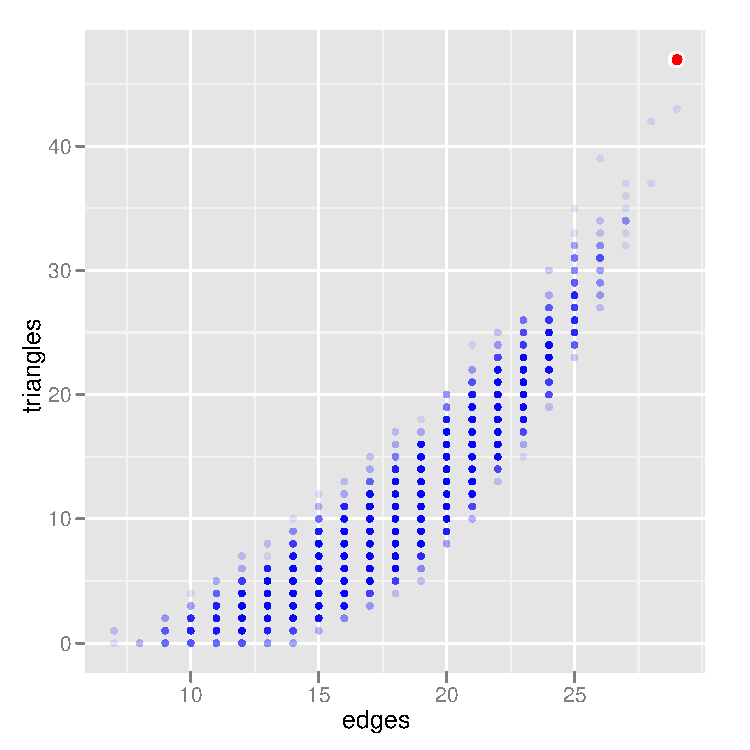
\includegraphics[width=\textwidth]{MCsample-bare} }}
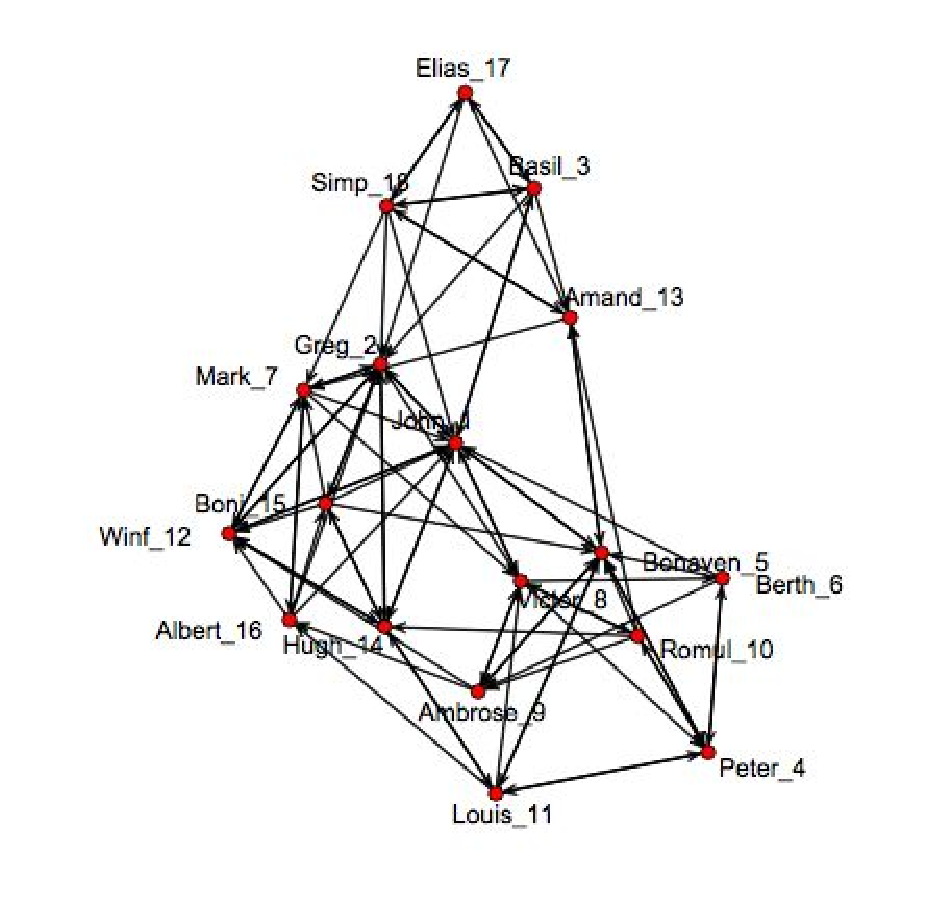
\includegraphics[width=1.5in]{samplike}
\end{column}

\begin{column}[r]{0.7\textwidth}
Use a simple model with only edges.  MLE can be 
found analytically,
\begin{align*}
	\etaMLE = -0.9072.
\end{align*}

\pause
MCMC-MLE may struggles to converge when
starting value $\eta_0$ is far from $\etaMLE$;

starting from $\eta_0 = 1$ took
10 iterations to converge (default in \texttt{ergm} package is three).
\end{column}
\end{columns}

\pause
We ran our algorithm starting at same $\eta_0=1$.  Our algorithm converged
after 21 iterations with 5 parameter updates.
{\footnotesize
\begin{table}
\begin{center}
\begin{tabular}{rrrrrrlrr}
  \hline
    &  &  &  & \multicolumn{1}{c}{inner}\\
  \multicolumn{1}{c}{$k$} & 
  \multicolumn{1}{c}{$\eta_k$} &
  \multicolumn{1}{c}{$\lVert \nabla \ell(\eta_k) \rVert$} &
  \multicolumn{1}{c}{$\alpha_k$} &
  \multicolumn{1}{c}{loop }\\
    &  &  &  & \multicolumn{1}{c}{count}\\
  \hline
   0 &  $1.0000$ & 135.64 &  0.012 & 8\\
   1 & $-0.6649$ & 15.99  &  0.014 & 2 \\
   2 & $-0.8817$ & 1.57   &  0.014 & 3 \\
   3 & $-0.9043$ & 0.22   &  0.012 & 8 \\
   4 & $-0.9069$ & 0.03   &  &  \\
   \hline
\end{tabular} \label{T:Sampson redo}
\end{center}
\end{table}}
}

\frame
{
  \frametitle{Example: large(ish) friendship network---1461 actors}  
 \setbeamercovered{transparent}
\begin{columns}[t]
\begin{column}[T]{0.3\textwidth}
%\includegraphics[height=1.5in]{g9-basic}
%\pgfputat{\pgfxy(0,0)}{\pgfbox[left,top]{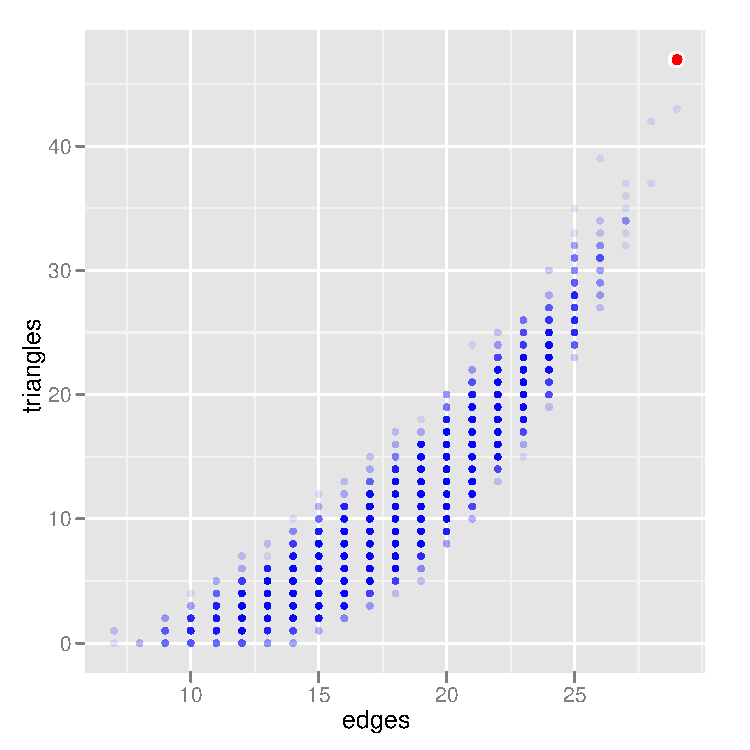
\includegraphics[width=\textwidth]{MCsample-bare} }}
\includegraphics[width=1.45in]{fmh-gradesex2}
\end{column}

\begin{column}[T]{0.7\textwidth}
Fit with a more realistic model that includes terms for \textbf{actor 
specific attributes} in addition to \textbf{network structures}.  
\vspace{1mm}

Actor specific attributes: Grade, Race, Sex.
\vspace{2mm}

Network structures: edges and geometrically weighted edgewise shared partners (GWESP)
\vspace{2mm}
\pause

Run our algorithm starting at $(0,0,0,0,0)$, compare to MCMC-MLE (starting at a value \emph{very close} to MLE).
\end{column}
\end{columns}
\vspace{2mm}

\pause
Stopped our algorithm after 40 $\eta_k$ updates over 144 iterations, taking 2hr 15min.
\begin{table}
\begin{center} 
%\caption[Comparison of MLEs for $\eta$ for MCMC-MLE and our algorithm for Faux Magnolia High example]{Comparison of MLEs for $\eta$ for MCMC-MLE and our algorithm for Faux Magnolia High example.  MCMC-MLE is the default algorithm
%in \texttt{ergm}, and is run here through 5 iterations starting
%at the MPLE ($\etaMLE$ below).
%Our algorithm is run for 40 steps ($\hat{\eta}_{\textrm{Steep}}$ below),
%starting from $(0,0,0,0,0)$.\\
%}

\begin{tabular}{rrrrrr}
  \hline
 & edges & Grade & Race & Sex & GWESP \\ 
  \hline
$\etaMLE$ & $-9.790$ & 2.755 & 0.906 & 0.780 & 1.813 \\ 
$\hat{\eta}_{\textrm{Steep}}$ & 	$-9.680$&	2.677&	0.875&	0.747&	1.818 \\ 
   \hline
\end{tabular}\label{T:FauxMagnolia}
\end{center}
\end{table}

Using smarter search directions (conjugate gradients) can get us closer even
faster.
}

\frame{
\frametitle{Updates on $\eta_k$}
{\tiny
\begin{table}
\begin{center} 
\begin{tabular}{rrrrrrr}
  \hline
  &  &  &  &  &  & \multicolumn{1}{c}{inner}\\
  \multicolumn{1}{c}{$k$} & 
  \multicolumn{1}{c}{$\eta[1]$} &
  \multicolumn{1}{c}{$\eta[2]$} &
  \multicolumn{1}{c}{$\eta[3]$} &
  \multicolumn{1}{c}{$\eta[4]$} &
  \multicolumn{1}{c}{$\eta[5]$} &
  \multicolumn{1}{c}{loop }\\
  &  & &  &  &  & \multicolumn{1}{c}{count}\\
\hline
% $k$&	$\eta[1]$&	$\eta[2]$&	$\eta[3]$&	$\eta[4]$& $\eta[5]$ \\%& $\nabla \ell(\eta_k)$\\
 \hline
0&	0& 0&	0&	0&	0 & - \\% &	89678.2 \\
1&	-2.279&	-0.393&	-1.265&	-1.138&	-2.675 & 2\\% &	24012.0 \\
2&	-4.051&	-0.56&	-1.686&	-1.314&	-2.646 & 2\\% &	4757.6\\
3&	-5.403&	-0.497&	-1.768&	-1.456&	-2.54 & 2\\% &	1125.5\\
4&	-7.321&	1.973&	0.224&	0.085&	-1.142 & 3\\% &	930.8\\
5&	-7.676&	1.872&	0.096&	-0.015&	-0.967 & 2\\% &	519.2\\
6&	-7.724&	2.187&	0.36	& 	0.234&	-0.476 & 3\\% &	771.5\\
7&	-7.996&	2.097&	0.259&	0.149&	-0.305 & 4\\% &	467.9\\
8&	-8.047&	2.373&	0.499&	0.368&	0.246 & 3\\% &	776.6\\
9&	-8.273&	2.274&	0.397&	0.28	&	0.387 & 4\\% &	421.9\\
10&	-8.33&	2.462&	0.565&	0.43	&	0.879 & 3\\% &	639.1\\
11&	-8.496&	2.38	& 	0.488&	0.364&	0.968 & 4\\% &	357.8\\
12&	-8.535&	2.468&	0.571&	0.439&	1.242 & 4\\% &	443.2\\
13&	-8.641&	2.416&	0.527&	0.403&	1.286 & 4\\% &	276.3\\
14&	-8.676&	2.462&	0.576&	0.449&	1.441 & 3\\% &	328.5\\
15&	-8.748&	2.427&	0.549&	0.428&	1.462 & 4\\% &	212.6\\
16&	-8.778&	2.456&	0.584&	0.462&	1.561 & 3\\% &	257.7\\
17&	-8.839&	2.429&	0.563&	0.448&	1.572 & 1\\% &	193.2\\
18&	-8.848&	2.449&	0.587&	0.471&	1.62	 & 3\\% &	175.5\\
19&	-8.907&	2.429&	0.575&	0.465&	1.637 & 3\\% &	171.5\\
20&	-8.913&	2.45	& 	0.599&	0.488&	1.676 & 2\\% &	154.6\\
21&	-8.953&	2.436&	0.591&	0.485&	1.683 & 2\\% &	130.3\\
22&	-8.965&	2.45	& 	0.61&	0.502&	1.713 & 3\\% &	111.9\\
23&	-9.047&	2.435&	0.608&	0.509&	1.739 & 3\\% &	199.4\\
24&	-9.042&	2.451&	0.625&	0.524&	1.758 & 3\\% &	82.7\\
...\\
%25&	-9.23&	2.45&	0.662&	0.576&	1.828&	229.1\\
%26&	-9.219&	2.469&	0.68	& 	0.592&	1.842&	52.5\\
%27&	-9.327&	2.484&	0.715&	0.622&	1.833&	191.9\\
%28&	-9.32&	2.496&	0.726&	0.631&	1.842&	41.4\\
%29&	-9.381&	2.535&	0.766&	0.669&	1.846&	117.1\\
%30&	-9.394&	2.53	& 	0.761&	0.664&	1.84	& 	33.0\\
%31&	-9.576&	2.603&	0.814&	0.718&	1.826&	128.8\\
%32&	-9.568&	2.614&	0.824&	0.725&	1.833&	18.3\\
%33&	-9.631&	2.662&	0.862&	0.748&	1.824&	94.5\\
%34&	-9.639&	2.656&	0.856&	0.742&	1.818&	28.0\\
%35&	-9.639&	2.657&	0.857&	0.743&	1.819&	12.8\\
%36&	-9.672&	2.678&	0.878&	0.751&	1.823&	35.6\\
%37&	-9.676&	2.677&	0.876&	0.749&	1.821&	33.3\\
38&	-9.678&	2.676&	0.875&	0.748&	1.819&	2\\%9.6\\
39&	-9.68&	2.677&	0.875&	0.747&	1.818 & 6\\% &	24.0\\
\hline
 $\etaMLE$ & -9.790 & 2.755 & 0.906 & 0.780 & 1.813 \\ [1ex] 

   \hline
\end{tabular}
\end{center}
\end{table}
}
%\textbf{Best use: from long range.  Then switch to faster algorithm.}
}





%%%%%%%%%%%%%%%%%%%%%%%%%%%%%%%%%%%%%%%%%%%%%%%%%%%%%%%%%%%%%
\section{non-Existent MLEs}
\frame
{
  \frametitle{Geyer, 2009}  
In 2009, Geyer woofed$^1$ about a way to handle non-existent MLEs in the case of generalized linear models.
\vspace{3mm}

\uncover<2->{
Log likelihood is a strictly concave function.  
\vspace{2mm}

For the MLE not to exist, there must be a direction $\delta$, called a  \textbf{generic direction of recession (GDOR)}, for which
$\ell(\eta + s\delta)$ is strictly increasing in $s$.
\vspace{3mm}

MLE is ``off at infinity" in the direction of $\delta$.
\vspace{5mm}

\uncover<3->{
Geyer (2009) showed how to 
\begin{itemize}
\item Check that MLE does not exist (in conventional sense).  In such a case, MLE exists in a limit of the distribution indexed by $\eta + s\delta$, $s \to +\infty$.
\vspace{1mm}

\uncover<4->{
\item Use this new information to construct one-sided confidence intervals for how close parameter $\eta$ is to infinity:
\begin{align*}
	[\hat{\eta}_L, +\infty)
\end{align*}
\end{itemize}
}

\vspace{0.2in}
}}
\footnotesize{$^1$Actually, Geyer had been woofing about MLE existence since at least as early as 1990.}
}


\frame
{
  \frametitle{Key ingredient: convex support}  
%   \setbeamercovered{transparent}
\begin{block}{Extension of Theorem 4 (Geyer, 2009)}
\begin{align*}
\text{MLE does not exist} \iff \text{a GDOR exists} \iff \text{$g(\yobs) \in$ relative boundary$(C)$}
\end{align*}
where  $C$ is the \emph{convex support} of the model.
\end{block}
\vspace{2mm}

The \textbf{convex support} $C$ is the smallest closed convex set that contains the natural statistics.
\vspace{2mm}

\pause
Need this to
\begin{itemize}
\item Determine MLE existence.
\item When MLE does not exist in conventional sense, find
\begin{itemize}
	\item	a GDOR $\delta$.
	\item 	MLE $\etaLCM$ in the limiting distribution.
\end{itemize}
	These give us what we need to calculate $[\hat{\eta}_L, +\infty)$.
\end{itemize}

}

\frame
{
  \frametitle{Conditions for non-existent MLE}  

\begin{columns}[T]
\begin{column}[T]{0.4\textwidth}
%\vspace{4mm}

{
Example: 9-node undirected network with edge and triangle statistics.
\vspace{1mm}

\begin{itemize}
\item 69 billion possible graphs in $\YY$.
\item Only 444 possible edge-triangle combinations.
\item $C$ is a 6-sided polytope.
\end{itemize}
\vspace{2mm}

\textbf{MLE exists if and only if
$g(\yobs)$ is in interior of $C$.}
}
\end{column}
\begin{column}[T]{0.6\textwidth}
%\begin{figure}
%\centering
\includegraphics[height=2.9in]{g9-hull}
%\caption{Convex support for 9-node undirected network model with edge and triangle
%statistics.}
%\label{F:g9-hull}
%\end{figure}
\end{column}
\end{columns}
}

%\frame
%{
%  \frametitle{Condition for non-existent MLE---theoretically}  
%\begin{theorem}[Extension of Theorem 4 (Geyer, 2009)]
%For a full exponential family with with log likelihood $\ell(\eta)$, convex support $C$, and observed data $\yobs$, the following are equivalent:
%\begin{enumerate}
%\item the MLE exists.
%\item Every direction of recession is direction of constancy.
%\item $N_C(g(\yobs))$ is a vector subspace.
%\item $T_C(g(\yobs))$ is a vector subspace.
%\item $g(\yobs) \in \rint C$.
%\end{enumerate}
%\end{theorem}
%}

\frame
{
	\frametitle{Observed data is $(31,50)$, on boundary.  Now what??}
%What is this ``limiting distribution"?
%\vspace{2mm}

Define a hyperplane $H$ passing through $g(\yobs)$, orthogonal to $\delta$.
\begin{columns}[]
\begin{column}[T]{0.45\textwidth}
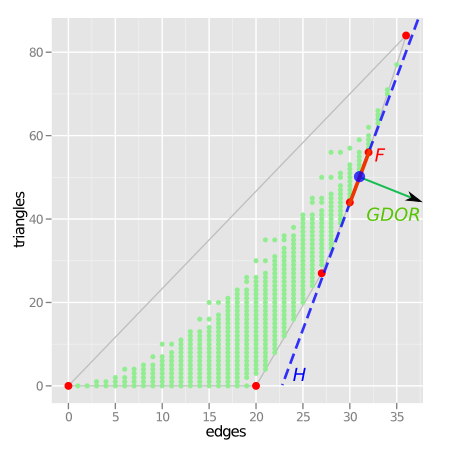
\includegraphics[height=2.2in]{g9-H.png}
\end{column}
\begin{column}[t]{0.57\textwidth}

\pause
By Theorem 6 (Geyer, 2009), as $s \to +\infty$,
\vspace{1mm}
\begin{itemize}
\item $P_{\eta + s \delta}( g(Y) \in H) \to 1.$
\vspace{1mm}

``Probability accumulates on the boundary."
\vspace{1mm}

\pause
\item $P_{\eta + s \delta}( Y = y) \to P_{LCM, \eta}( Y = y)$.
\vspace{1mm}

The limiting distribution is called the \textbf{limiting conditional model (LCM)}.
\end{itemize}
\end{column}
\end{columns}
}

\frame
{
	\frametitle{Limiting conditional model}
\begin{columns}[]
\begin{column}[T]{0.25\textwidth}
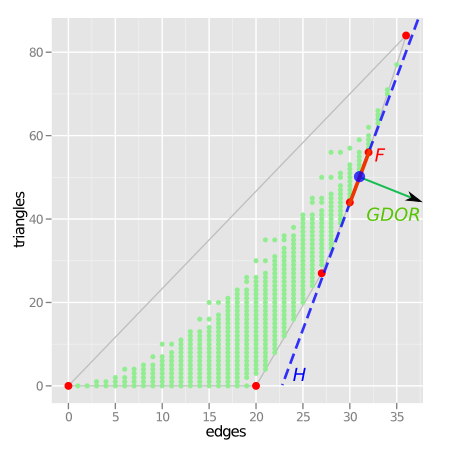
\includegraphics[height=2.2in,trim=3.5in 2in 0.15in 0.05in,clip=true]{g9-H.png}
\end{column} % l b r t

\begin{column}[t]{0.75\textwidth}
$P_{\eta + s \delta}( Y = y) \to \alert{P_{LCM, \eta}( Y = y)}$ as $s \to +\infty$.
\begin{block}{
By Theorem 6 (Geyer, 2009)}
\begin{itemize}
	\item $\alert{P_{LCM, \eta}( Y = y)} = P_{\eta}( Y =y \mid g(Y) \in H)$.
\vspace{1mm}
	
	%It is the conditional distribution of $Y \mid g(Y) \in H$ with parameter $\eta.$
	\item it is an exponential family with convex support $C \cap H$.
\vspace{1mm}

	\item the MLE for this LCM, $\etaLCM$, is guaranteed to exists.
\vspace{1mm}

	\item $\ell(\eta) < \ell_{LCM}(\eta)$.
\end{itemize}
\end{block}

\end{column}
\end{columns}
}


\frame
{
  \frametitle{Measuring closeness to infinity}  
So,
\begin{align*}
	\lim_{s \to +\infty} \ell(\etaLCM + s\delta) = \sup_{\eta \in \RR^d} \ell(\eta).
\end{align*}	

MLE for original model: off at $+\infty$.

Now, some more detail: it is $\etaLCM$ sent to infinity in direction of $\delta$.
\vspace{2mm}


\emph{Can we say anything about how close $\eta$ is to infinity?  }
\vspace{2mm}

\pause
Find unique $s$, $\hat{s}$, such that
\begin{align*}
		P_{\etaLCM + s \delta}( g(Y) \in H) = \alpha.
\end{align*}
%Then $[ \hat{s}, +\infty)$ is a $1- \alpha$ confidence interval for the parameter $s$, 
\pause
Then
\begin{align*}
[ \etaLCM + \hat{s} \delta, + \infty)
\end{align*}
gives a $1 - \alpha$ confidence region for the parameter $\etaLCM + s \delta$.
\vspace{3mm}

\pause
\begin{block}{}
Find $\etaLCM$ and a GDOR $\delta$.
\end{block}
}

%\frame
%{
%  \frametitle{Previous work}  
%
%\begin{columns}[t]
%%
%\begin{column}[2in]
%Handcock (2003), Rinaldo, Fienberg, and Zhou (2009).
%\end{column}
%
%\begin{column}[4in]
%\begin{figure}[h]
%\centering
%\includegraphics[height=2.6in]{g9-hull}
%\caption{Convex support for 9-node network model with edge and triangle
%statistics.}
%%\label{F:g9-hull}
%\end{figure}
%\end{column}
%\end{columns}
%}
\frame
{
  \frametitle{Previous work}  
Handcock (2003), Rinaldo, Fienberg, and Zhou (2009) studied 7 and 9-node undirected networks
with two statistics.
\begin{itemize}
	\item Confirmed condition for relative location of $g(\yobs)$ for MLE to not exist.  
	%That is, found face of $C$ in which $g(\yobs)$ lies in relative interior.
	\item Identified cones that bound DORs.% (normal cones of $C$ at $g(\yobs)$).
\end{itemize}
\pause
Authors use full knowledge of convex support of model $C$ to determine above.

\begin{columns}[]
\begin{column}[T]{0.4\textwidth}
\includegraphics[width=1.8in]{g9-basic}
\end{column}

\begin{column}[t]{0.6\textwidth}

In particular, H-representation of $C$:
\begin{align*}
	Ax \leq b.
\end{align*}
Easy to check if a point is in exterior, interior, or boundary of hull.

\end{column}
\end{columns}

\pause
\textbf{But in a real problem, we don't have this!}

}

%%%%%%%%%%%%%%%%%%%%%%%%%%%%%%%%%%%%%%%%%%%%%%%%%%%%%%%%%%%%%
\section{Algorithm extended}
\frame
{
\frametitle{What do we have?}
MCMC samples from distribution with parameter $\eta_k$.  

And here, we're trying to do more: determine if MLE exists, and if not, find $\etaLCM$ and 
a GDOR $\delta$.
\vspace{1ex}

\begin{columns}[t]
\begin{column}[T]{0.4\textwidth}
%\includegraphics[height=1.5in]{g9-basic}
%\pgfputat{\pgfxy(0,0)}{\pgfbox[left,top]{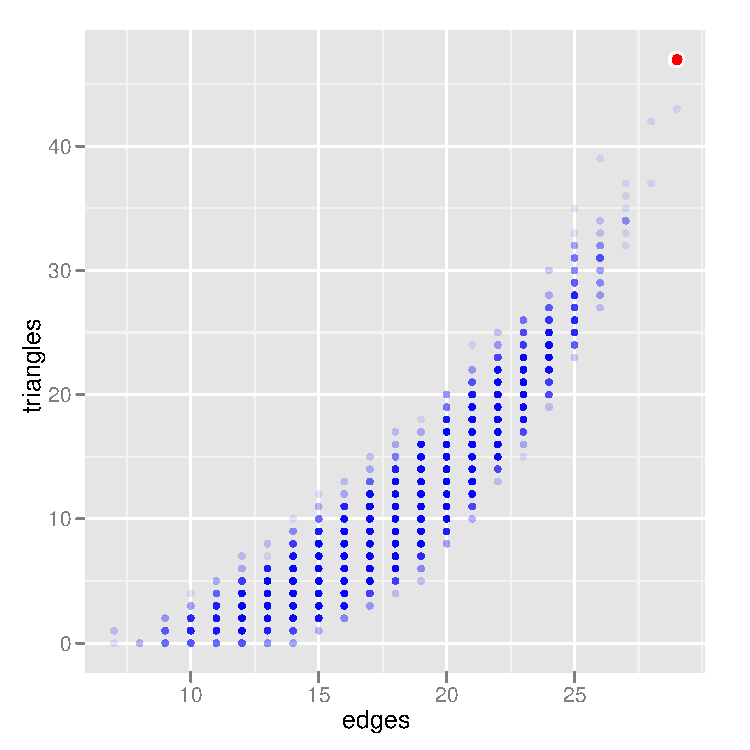
\includegraphics[width=\textwidth]{MCsample-bare} }}
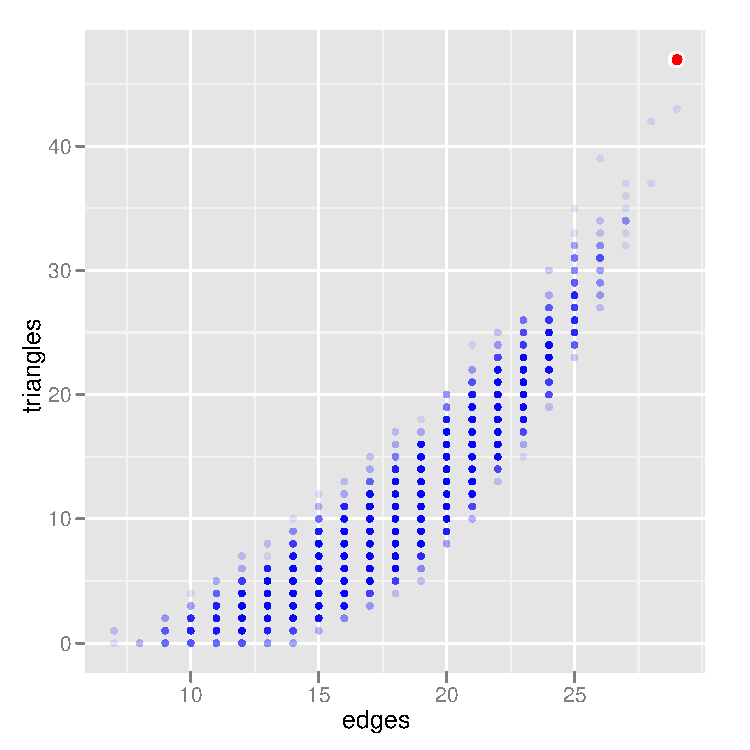
\includegraphics[width=2in]{MCsample-bare}
\end{column}

\begin{column}[r]{0.6\textwidth}
\pause

\begin{itemize}
\item But that's all we needed to find the MLE before! 
%\vspace{1mm}


\item Iterated sampling from distribution with parameter $\eta_k$ until $\nabla \ell(\eta_k) = 0$.

Or alternatively, until
\begin{align*}
	\E_{\eta_k} g(Y) = g(\yobs).
\end{align*}

\end{itemize}
\end{column}
\end{columns}
}

\frame
{
\frametitle{Case: MLE exists}  
\begin{figure}[h]
\centering
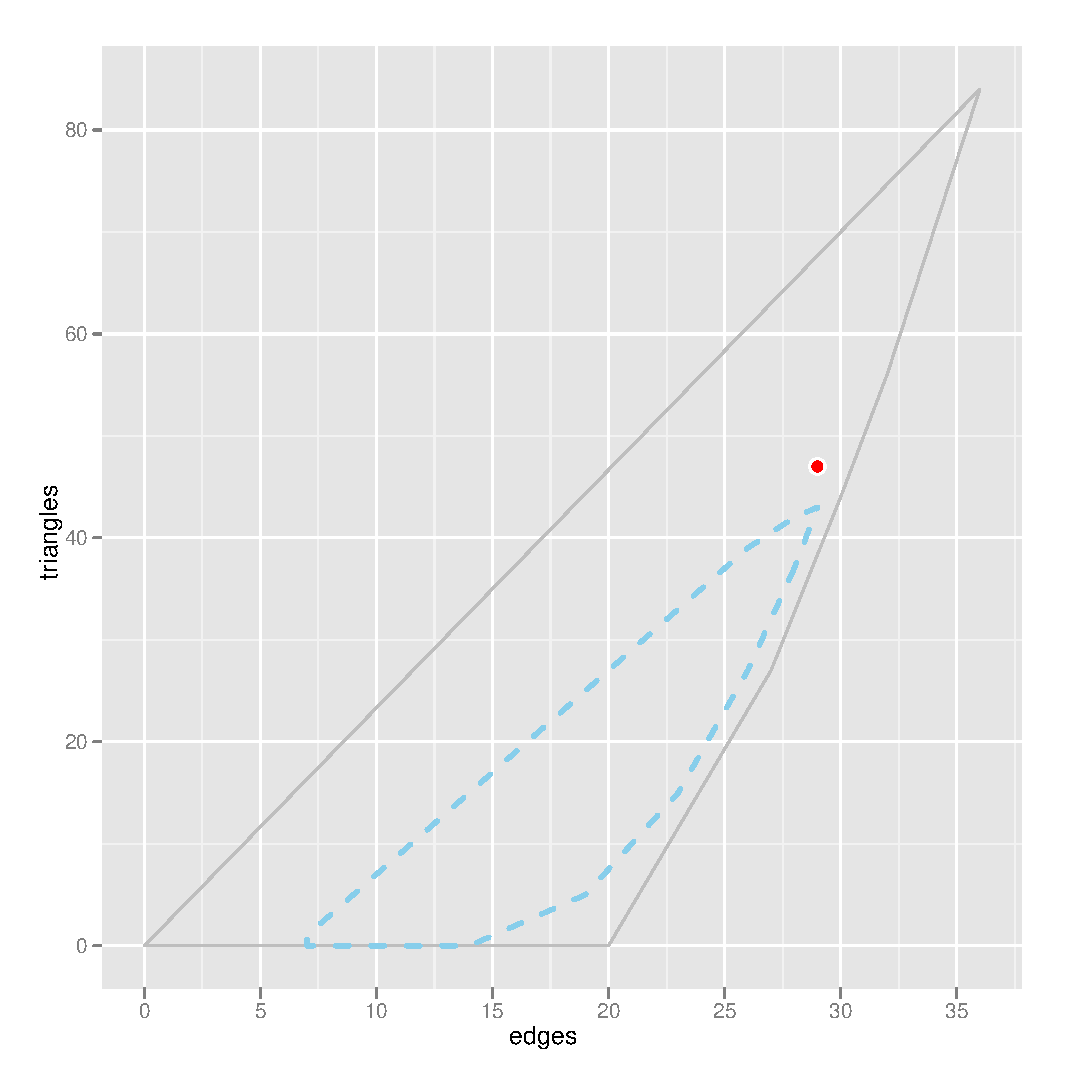
\includegraphics[height=2.2in]{MCsample-far}
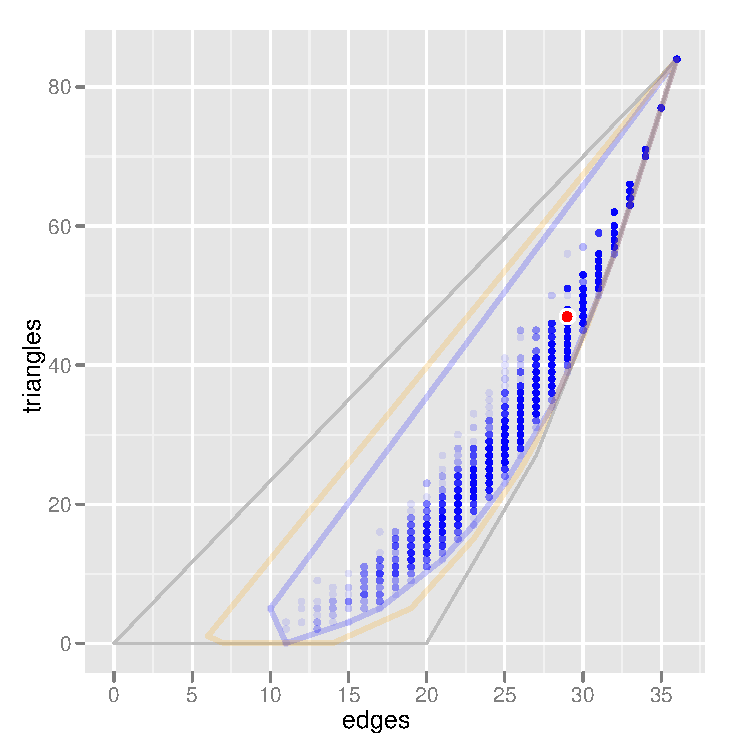
\includegraphics[height=2.2in]{MCsample-MLE}
\caption{MCMC samples from distributions with $\eta = (0,0)$ (left), and $\eta=\etaMLE$ (right).}
\label{F:MCsample-MLE exists}
\end{figure}
%MCMC samples from distributions with $\eta = (0,0)$ (left), and $\eta=\etaMLE$ (right).
}


\frame
{
\frametitle{Extend our algorithm}  
\textbf{Idea}: Use MCMC samplers to explore space of natural statistics and
determine geometry of convex support $C$.
\vspace{2mm}
\pause

\includegraphics[height=1.3in]{minesweeper}
\vspace{2mm}

\pause
Our algorithm climbs up log likelihood.  So we know that cloud of points will move towards $g(\yobs)$.
\vspace{2mm}
\pause

Find a way to determine if
\begin{enumerate}
\item $g(\yobs)$ is on the boundary of our sample hull.
\item If so, on what face of our sample hull does it lie?
\item Is the boundary of the sample hull also the boundary of $C$?
\end{enumerate}
}

\frame
{
\frametitle{Case: MLE does not exists}  
\begin{figure}[h]
\centering
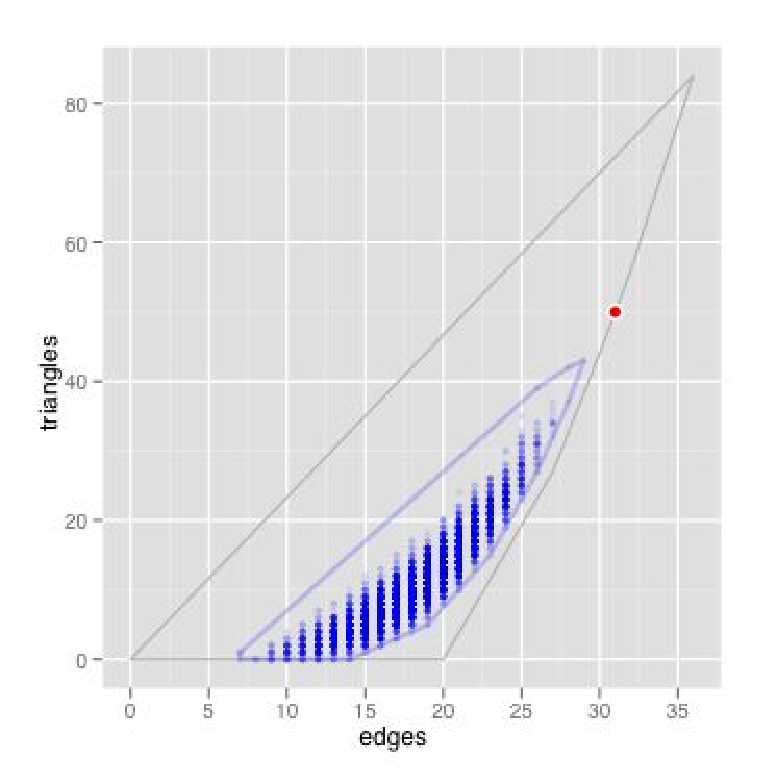
\includegraphics[height=2.2in]{MCsample-boundary}
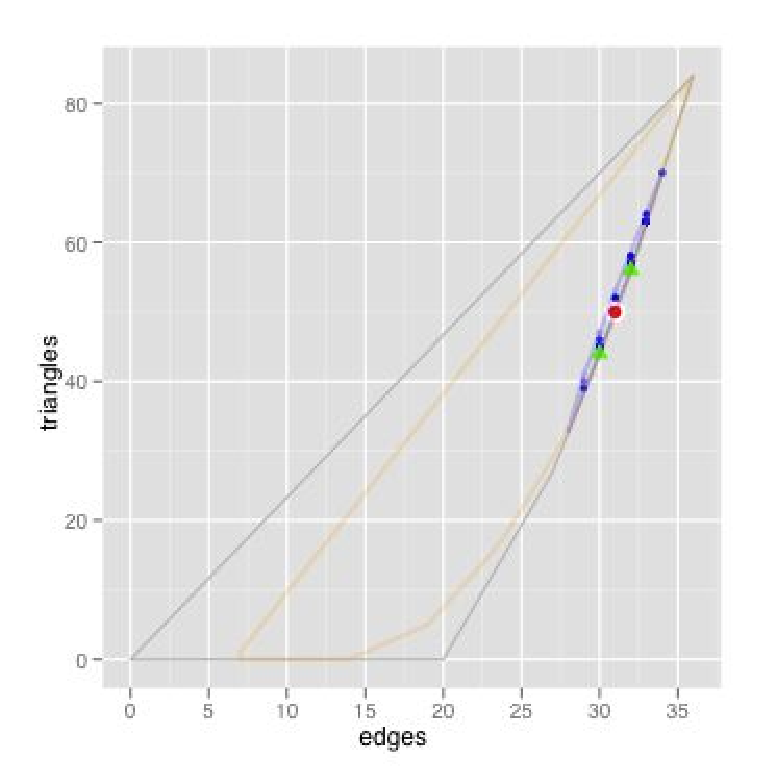
\includegraphics[height=2.2in]{MCsample-77face}
%\caption{MCMC samples from distributions with $\eta = (0,0)$ (left), and 
%when $\eta$ is close to MLE in LCM (right).}
\label{F:MCsample-MLE nonexistent}
\end{figure}
}

\frame
{
\setbeamercovered{transparent}

\frametitle{\texttt{rcdd} to the rescue}  
These are problems in \emph{computational geometry}.  

Fortunately, the \texttt{rcdd} package (Geyer and Meeden, 2009) has the 
linear programming tools we need to answer these questions.

\begin{columns}[T]
\begin{column}[T]{0.25\textwidth}
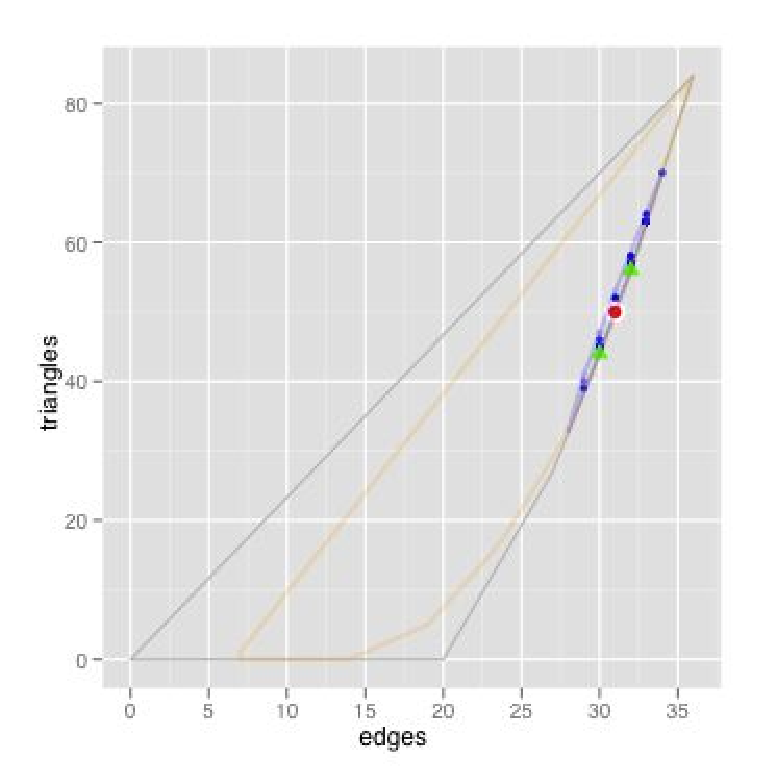
\includegraphics[height=2.5in,trim=3.5in 2in 0.15in 0.05in,clip=true]{MCsample-77face} % l b r t
\end{column}
\begin{column}[T]{0.75\textwidth}
\vspace{2mm}

\begin{enumerate}
\item $g(\yobs) \notin$ sample hull.  

\uncover<2->{
\emph{Check for existence of a strongly separating hyperplane using \texttt{lpcdd}.}
}
\item Find face $F$ on which $g(\yobs)$ lies in relative interior.  

\uncover<2->{
\emph{Use \texttt{linearity} function.}
}
\item Find a GDOR $\delta$ orthogonal to $F$.  

\uncover<2->{
\emph{Set up and solve a linear programming problem
using \texttt{lpcdd} to return a $\delta$.}  

Here, $\delta = (6,-1)$.
\alert{(GDOR \checkmark)}
}
\end{enumerate}
\uncover<3->{
\textbf{Can do all these using rational arithmetic and without calculating expensive H-representations of hulls.}
}
\end{column}
\end{columns}
}

%\frame
%{
%\frametitle{When is our boundary \emph{the} boundary?}  
%\setbeamercovered{transparent}
%
%\begin{columns}[T]
%\begin{column}[T]{0.25\textwidth}
%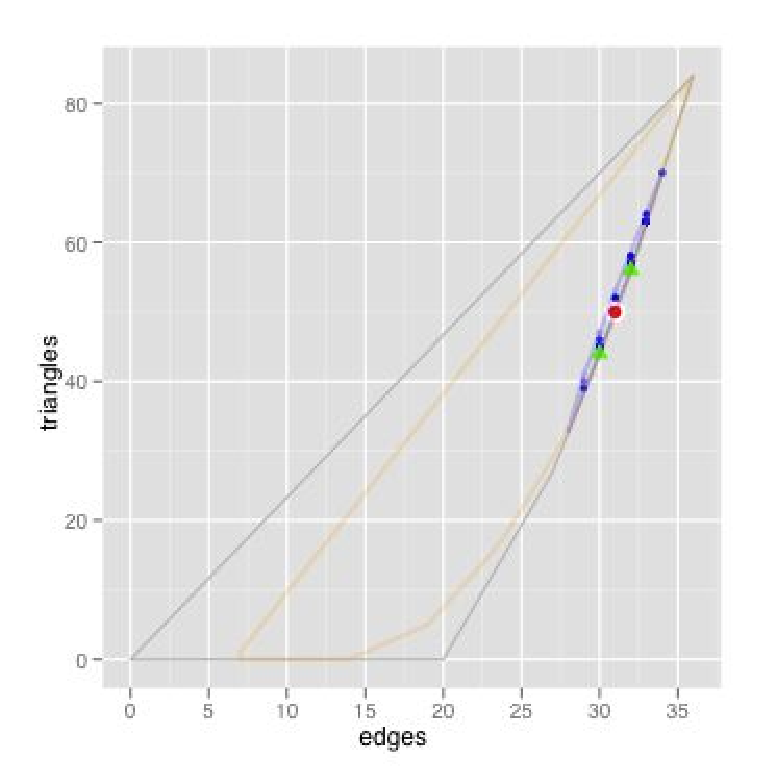
\includegraphics[height=2.5in,trim=3.5in 2in 0.15in 0.05in,clip=true]{MCsample-77face} % l b r t
%\end{column}
%
%\begin{column}[T]{0.75\textwidth}
%One thing we can't get from \texttt{rcdd}: 
%
%tell us if $F$ of the hull 
%of our samples is also on the boundary of $C$.  
%\vspace{2mm}
%
%\textbf{Our approach:} if $>60\%$ of samples land on our empirical $F$, then $F$ is on the boundary.
%\vspace{4mm}
%
%\pause
%Here, 77\% of the samples fall on three points (including $g(\yobs)$) that define $F$.  
%\vspace{2mm}
%
%\textbf{Conclude (correctly) that $F$ is a boundary of $C$.}
%\end{column}
%\end{columns}
%}


\frame
{
\setbeamercovered{transparent}
\frametitle{One-sided CI?}  
Still need MLE $\etaLCM$ for LCM.
\pause

Earlier theorem says $F$ (which we just found) is the support for LCM.
So, with small adjustment to support, can use our same algorithm to find $\etaLCM$!   \checkmark!
\vspace{2mm}
\begin{align*}
	\etaLCM = (126.8, -21.1)
\end{align*}

Finally, one-sided CI.
\pause

Find unique $s$, call it $\hat{s}$, such that
\begin{align*}
		P_{\etaLCM + s \delta}( g(Y) \in H) = \alpha.
\end{align*}
Then $1- \alpha$ confidence interval is
\begin{align*}
[ \etaLCM + \hat{s} \delta, + \infty)
\end{align*}

In this example, we calculate a non-simultaneous 95\% confidence region
\begin{align*}
	[9.145, +\infty) \\
	(-\infty, -1.500].
\end{align*}
}
%%%%%%%%%%%%%%%%%%%%%%%%%%%%%%%%%%%%%%%%%%%%%%%%%%%%%%
\section{Next steps}
\frame
{
\frametitle{Done.  For the moment.}
Thoughts
\begin{itemize}
	\item Parameter is an index to a distribution.  Goal is the distribution, not the number.
\end{itemize}


Next steps
\begin{itemize}
	\item Switch criteria, from our algorithm to MCMC-MLE
	\item Step length search
	\item Proof of convergence for noisy $\nabla \ell( \eta)$.
\end{itemize}
}



%%%%%%%%%%%%%%%%%%%%%%%%
\appendix
\newcounter{finalframe}
\setcounter{finalframe}{\value{framenumber}}
% Backup frames





\frame
{
\frametitle{When is our boundary \emph{the} boundary?}  
\setbeamercovered{transparent}

\begin{columns}[T]
\begin{column}[T]{0.25\textwidth}
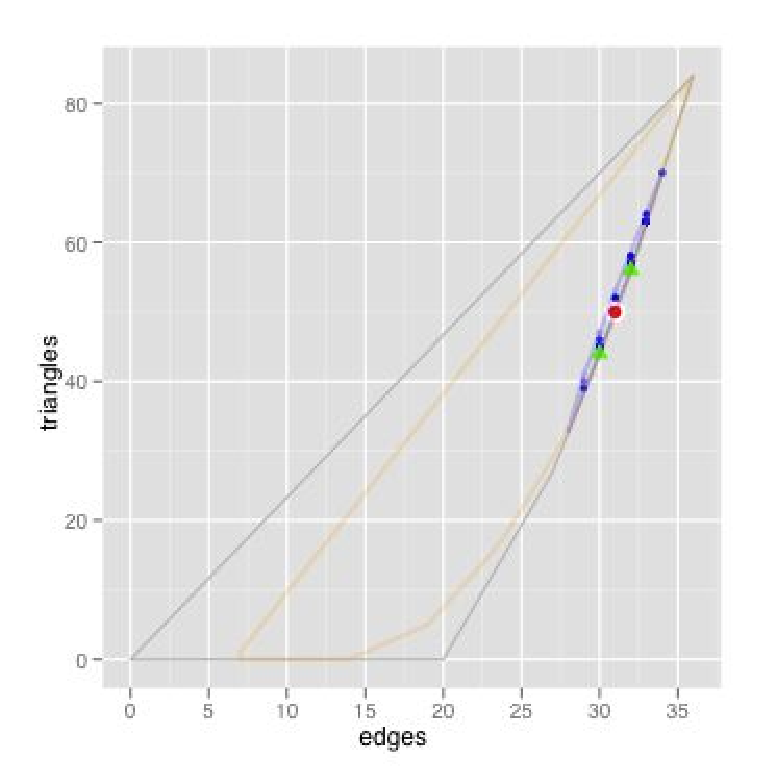
\includegraphics[height=2.5in,trim=3.5in 2in 0.15in 0.05in,clip=true]{MCsample-77face} % l b r t
\end{column}

\begin{column}[T]{0.75\textwidth}
One thing we can't get from \texttt{rcdd}: 

tell us if $F$ of the hull 
of our samples is also on the boundary of $C$.  
\vspace{2mm}

\textbf{Our approach:} if $>60\%$ of samples land on our empirical $F$, then $F$ is on the boundary.
\vspace{4mm}

%\pause
Here, 77\% of the samples fall on three points (including $g(\yobs)$) that define $F$.  
\vspace{2mm}

\textbf{Conclude (correctly) that $F$ is a boundary of $C$.}

MLE therefore does not exist in conventional sense (\checkmark).

\end{column}
\end{columns}
}
\frame
{
\frametitle{Case: MLE exists, but observed data close to boundary}  
\begin{figure}[h]
\centering
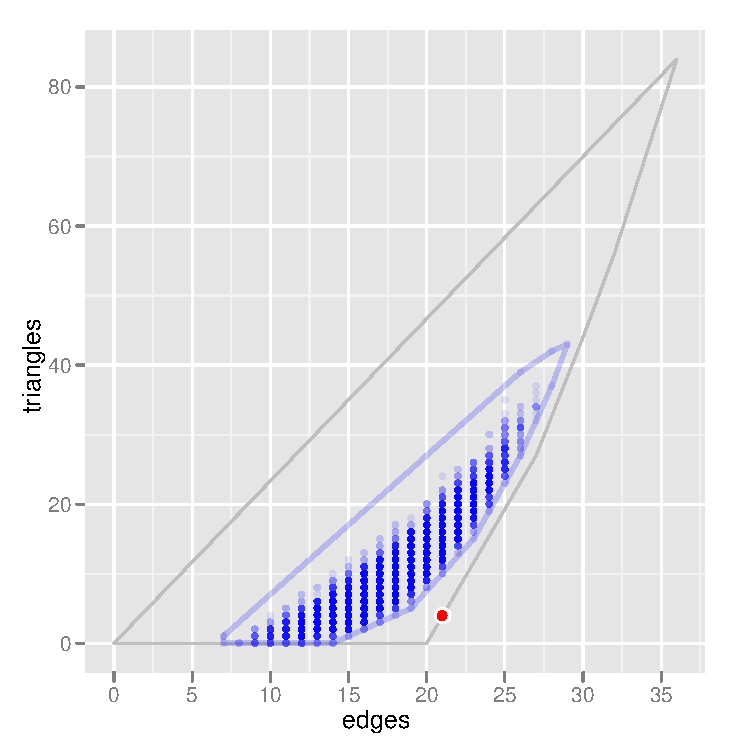
\includegraphics[height=2.5in]{MCsample-problem}
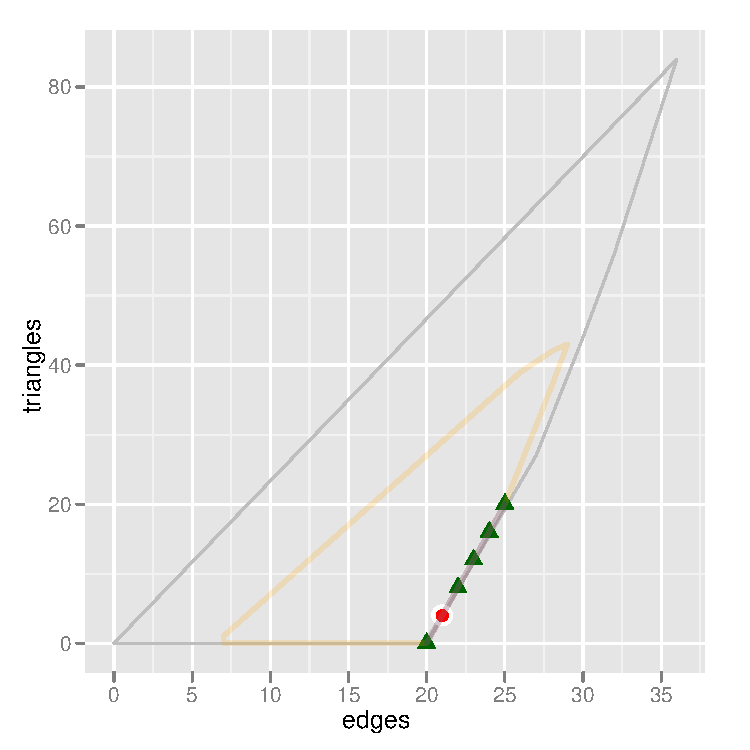
\includegraphics[height=2.5in]{MCsample-fakeface}
\caption{MCMC samples when MLE does not exist.}
\label{F:MCsample-MLE problem}
\end{figure}
}
\setcounter{framenumber}{\value{finalframe}}

\end{document}
